\documentclass[11pt]{article}
\usepackage{enumerate}
\usepackage{fullpage}
\usepackage{fancyhdr}
\usepackage{amsmath, amsfonts, amsthm, amssymb}
\usepackage{color}
\usepackage[]{graphicx}
\setlength{\parindent}{0pt}
\setlength{\parskip}{5pt plus 1pt}
\pagestyle{empty}

\def\indented#1{\list{}{}\item[]}
\let\indented=\endlist

\newcounter{questionCounter}
\newcounter{partCounter}[questionCounter]
\newenvironment{question}[2][\arabic{questionCounter}]{%
    \setcounter{partCounter}{0}%
    \vspace{.25in} \hrule \vspace{0.5em}%
        \noindent{\bf #2}%
    \vspace{0.8em} \hrule \vspace{.10in}%
    \addtocounter{questionCounter}{1}%
}{}
\renewenvironment{part}[1][\alph{partCounter}]{%
    \addtocounter{partCounter}{1}%
    \vspace{.10in}%
    \begin{indented}%
       {\bf (#1)} %
}{\end{indented}}

%%%%%%%%%%%%%%%%%%%%%%%HEADER%%%%%%%%%%%%%%%%%%%%%%%%%%%%%%
\newcommand{\myname}{Shashank Singh}
\newcommand{\myandrew}{sss1@andrew.cmu.edu}
\newcommand{\myclass}{15-423 Digital Signal Processing for CS}
\newcommand{\myhwnum}{2}
\newcommand{\duedate}{Wednesday, February 13, 2013}
%%%%%%%%%%%%%%%%%%%%%%%%%%%%%%%%%%%%%%%%%%%%%%%%%%%%%%%%%%%

%%%%%%%%%%%%%%%%%%%%CONTENT MACROS%%%%%%%%%%%%%%%%%%%%%%%%%
\renewcommand{\qed}{\quad $\blacksquare$}
\newcommand{\mqed}{\quad \blacksquare}
\newcommand{\inv}{^{-1}}
\newcommand{\argmax}{\operatornamewithlimits{argmax}}
\newcommand{\argmin}{\operatornamewithlimits{argmin}}
\newcommand{\N}{\mathbb{N}} % natural numbers
\newcommand{\Z}{\mathbb{Z}} % natural numbers
\newcommand{\Q}{\mathbb{Q}} % rational numbers
\newcommand{\R}{\mathbb{R}} % real numbers
\newcommand{\sminus}{\backslash} % asymmetric set difference
\newcommand{\e}{\varepsilon} % \varepsilon
\newcommand{\I}{\mathcal{I}}

% probability related macros
\newcommand{\pr}[1]{\mathsf{P}\left( #1 \right)} % probability of event #1
\newcommand{\E}[2]{\operatornamewithlimits{\mathbb{E}}_{#2}\left[ #1 \right]} % expected value of #1 over #2
\newcommand{\Bern}[1]{\operatorname{Bernoulli}\left( #1 \right)} % Bernoulli distribution of parameter p
\newcommand{\giv}{\, | \,} % \pr{A \giv B} probability of A given B
%%%%%%%%%%%%%%%%%%%%%%%%%%%%%%%%%%%%%%%%%%%%%%%%%%%%%%%%%%%

\begin{document}
\thispagestyle{plain}

{\Large Homework \myhwnum} \\
\myclass \\
Name: \myname \\
Email: \myandrew \\
Due: \duedate

\section{Proof}
By definition of the convolution,
$\forall n \in \Z$,
\begin{align*}
((x \otimes h_1) \otimes h_2)[n]
 & = \sum_{j = -\infty}^{\infty} (x \otimes h_1)[n - j] h_2[j] \\
 & = \sum_{j = -\infty}^{\infty} \left( \sum_{k = -\infty}^{\infty}
                                         x[k] h_1[n - j - k]\right) h_2[j] \\
 & = \sum_{k = -\infty}^{\infty} x[k] \sum_{j = -\infty}^{\infty}
                                                     h_1[n - j - k] h_2[j] \\
 & = \sum_{k = -\infty}^{\infty} x[k] (h_1 \otimes h_2)[n - k]
   = (x \otimes (h_1 \otimes h_2))[n]. \mqed
\end{align*}

\section{Convolutions}
\begin{enumerate}
\item By definition of the convolution, $\forall n \in \Z$,
\[
  (x \otimes h)[n]
 = \sum_{k = -\infty}^{\infty} u[n - k] u[k] \alpha^k
 = \sum_{k = 0}^{n} \alpha^k
 = \mbox{\fbox{$\displaystyle
        \left\{
            \begin{array}{cl}
                \frac{1 - \alpha^{n + 1}}{1 - \alpha} & : n \geq 0 \\
                0                                     & : n < 0
            \end{array}
        \right.
$.}}
\]
See Figure~\ref{fig:2.1} for graph.
\begin{figure}[h]
\begin{center}
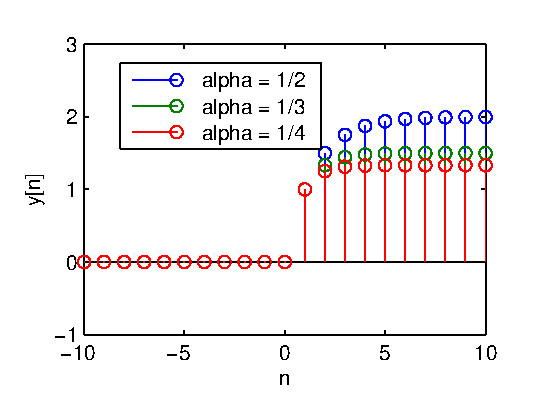
\includegraphics[width=0.46\textwidth]{2.1.eps}
\end{center}
\caption{$y[n] = (x \otimes h)[n]$ plotted for $n \in [-10,10]$ and for various
values of $\alpha$.}
\label{fig:2.1}
\end{figure}

\item By definition of the convolution, $\forall t \in \R$,
\[
  (x \otimes h)(t)
 = \int_{-\infty}^{\infty} u(t - s)u(s)e^{\alpha s} \, ds
 = \int_0^t e^{\alpha s} \, ds
 = \frac{e^{\alpha s}}{\alpha} \bigg|_{s = 0}^{s = t}
 = \mbox{\fbox{$\displaystyle
        \left\{
            \begin{array}{cl}
                \frac{e^{\alpha t} - 1}{\alpha} & : t \geq 0 \\
                0                               & : t < 0
            \end{array}
        \right.
$.}}
\]
See Figure~\ref{fig:2.2} for graph.
\begin{figure}[h]
\begin{center}
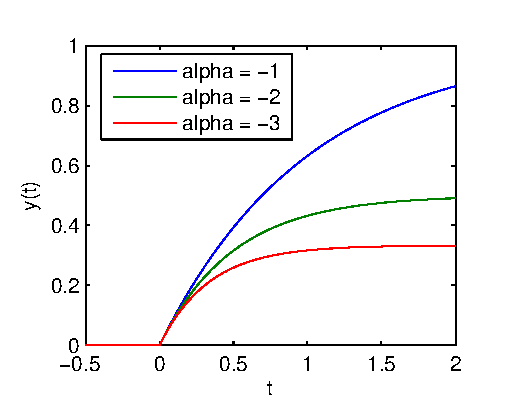
\includegraphics[width=0.46\textwidth]{2.2.eps}
\end{center}
\caption{$y(t) = (x \otimes h)(t)$ plotted for $t \in [-0.5,2]$ and for various
values of $\alpha$.}
\label{fig:2.2}
\end{figure}
 
\item By definition of the convolution, $\forall n \in \N$,
\[
(x \otimes h)[n]
 = \sum_{k = -\infty}^{\infty} u[n]u[n - k]
 = \sum_{k = 0}^n 1
 = \mbox{\fbox{$\displaystyle
        \left\{
            \begin{array}{cl}
                n & : n \geq 0 \\
                0 & : n < 0
            \end{array}
        \right.
$.}}
\]
See Figure~\ref{fig:2.3} for graph.
\begin{figure}[h]
\begin{center}
\includegraphics[width=0.46\textwidth]{2.3.eps}
\end{center}
\caption{$y[n] = (x \otimes h)[n]$ plotted for $n \in [-10,10]$.}
\label{fig:2.3}
\end{figure}
 
\item Note that, $\forall n \in \N$, $x[n] = u[n] - u[n - n_0]$ and
$h[n] = u[n] - u[n - n_1]$.

Linearity allows us to distribute the convolution over the differences, and
then shift-invariance allows us to compute all of the resulting convolutions as
shifted versions of the convoluion computed in Problem 3.
Thus, $\forall n \in \N$, we have
\[
(x \otimes h)[n]
 = \mbox{\fbox{$\displaystyle
        \left\{
            \begin{array}{cl}
                0 & : n \leq 0                              \\
                n & : 0 < n \leq n_1                        \\
                n - (n - n_1) = n_1 & : n_1 < n \leq n_2    \\
                n_1 - (n - n_2) = n_1 + n_2 - n & : n < 0
            \end{array}
        \right.
$.}}
\]
See Figure~\ref{fig:2.4} for graph.
\begin{figure}[h]
\begin{center}
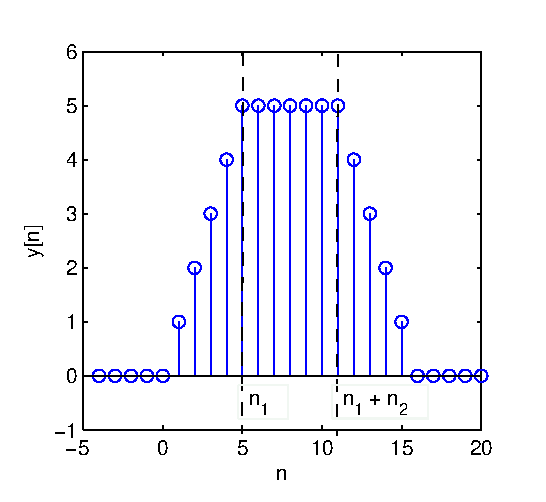
\includegraphics[width=0.46\textwidth]{2.4.eps}
\end{center}
\caption{$y[n] = (x \otimes h)[n]$ plotted for $n \in [-5,20]$, with $n_1 = 5$
and $n_2 = 6$.}
\label{fig:2.4}
\end{figure}

\item Note that, $\forall n \in \N$, $x[n] = u[n] - u[n - n_0]$.
By definition of convolution, $\forall n \in \N$,
\begin{align*}
(x \otimes h)[n]
 & = \sum_{k = -\infty}^{\infty} (u[n - k] - u[n - n_0 - k])u[k]\alpha^k
   = \sum_{k = 0}^n \alpha^k - \sum_{k = 0}^{n - n_0} \alpha^k \\
 & = \mbox{\fbox{$\displaystyle
        \left\{
            \begin{array}{cl}
                \frac{\alpha^{n + 1} - \alpha^{n - n_0 + 1}}{\alpha - 1} & :
n_0 < n \\
                \frac{\alpha^{n + 1} - 1}{\alpha - 1} & : 0 < n \leq n_0 \\
                0 & : n \leq 0
            \end{array}
        \right.
$.}}
\end{align*}
\end{enumerate}
\end{document}
